% !TeX program = pdfLaTeX
\documentclass[12pt]{article}
\usepackage{amsmath}
\usepackage{graphicx,psfrag,epsf}
\usepackage{enumerate}
\usepackage{natbib}
\usepackage{textcomp}
\usepackage[hyphens]{url} % not crucial - just used below for the URL
\usepackage{hyperref}

%\pdfminorversion=4
% NOTE: To produce blinded version, replace "0" with "1" below.
\newcommand{\blind}{0}

% DON'T change margins - should be 1 inch all around.
\addtolength{\oddsidemargin}{-.5in}%
\addtolength{\evensidemargin}{-.5in}%
\addtolength{\textwidth}{1in}%
\addtolength{\textheight}{1.3in}%
\addtolength{\topmargin}{-.8in}%

%% load any required packages here



% tightlist command for lists without linebreak
\providecommand{\tightlist}{%
  \setlength{\itemsep}{0pt}\setlength{\parskip}{0pt}}



\usepackage[dvipsnames]{xcolor} % colors
\newcommand{\aak}[1]{{\textcolor{blue}{#1}}}
\newcommand{\svp}[1]{{\textcolor{RedOrange}{#1}}}
\newcommand{\yg}[1]{{\textcolor{Green}{#1}}}
\usepackage[capitalise]{cleveref}
\newcommand\pcref[1]{(\cref{#1})}
\usepackage{algorithm,algpseudocode,booktabs}
\usepackage{booktabs}
\usepackage{longtable}
\usepackage{array}
\usepackage{multirow}
\usepackage{wrapfig}
\usepackage{float}
\usepackage{colortbl}
\usepackage{pdflscape}
\usepackage{tabu}
\usepackage{threeparttable}
\usepackage{threeparttablex}
\usepackage[normalem]{ulem}
\usepackage{makecell}
\usepackage{xcolor}

\begin{document}


\def\spacingset#1{\renewcommand{\baselinestretch}%
{#1}\small\normalsize} \spacingset{1}


%%%%%%%%%%%%%%%%%%%%%%%%%%%%%%%%%%%%%%%%%%%%%%%%%%%%%%%%%%%%%%%%%%%%%%%%%%%%%%

\if0\blind
{
  \title{\bf A Spatio-Temporal Model for Arctic Sea Ice}

  \author{
        Alison Kleffner 1 \\
    Department of Statistics, University of Nebraska - Lincoln\\
     and \\     Susan VanderPlas 2 \\
    Department of Statistics, University of Nebraska - Lincoln\\
     and \\     Yawen Guan 3 \\
    Department of Statistics, University of Nebraska - Lincoln\\
      }
  \maketitle
} \fi

\if1\blind
{
  \bigskip
  \bigskip
  \bigskip
  \begin{center}
    {\LARGE\bf A Spatio-Temporal Model for Arctic Sea Ice}
  \end{center}
  \medskip
} \fi

\bigskip
\begin{abstract}
Arctic Sea Ice is a barrier between the warm air of the ocean and the
atmosphere, thus playing an important role in the climate. When narrow
linear cracks (leads) form in the sea ice, the heat from the ocean is
then released into the atmosphere. To estimate where cracks may form,
motion data from the RADARSAT Geophysical Processing System (RGPS) are
analyzed. The RGPS provides a set of trajectories (or cells) to trace
the displacements of sea ice, however, chunks of data are missing due to
the data collection method. We propose a spatial clustering and
interpolation method that allows us to infer missing observations and
estimate, where a crack may form. To do this feature inputs were created
for KNN clustering by creating a bounding box around each trajectory,
resulting in trajectories being assigned a cluster. A crack is
considered to have formed on the boundary between different clusters.
Within the clusters, spatiotemporal interpolation method is used to
infer missing locations. Our clustering approach is then compared to
other methods to determine ice crack formation, and cross-validation is
used to assess our interpolation method.
\end{abstract}

\noindent%
{\it Keywords:} spatial clustering, non-stationary, Gaussian process.
\vfill

\newpage
\spacingset{1.45} % DON'T change the spacing!

\hypertarget{introduction}{%
\section{Introduction}\label{introduction}}

Sea ice is frozen sea water in the Arctic Ocean that generally occurs as
an ice pack which can drift over the ocean surface. When it is
stationary, it acts as an insulator between the warm ocean and the
cooler atmosphere \citep{peterson_evaluating_2011}. However, sea ice is
constantly changing and moving due to dynamic thermodynamic and dynamic
processes \citep{hutter_leads_2019}. These processes, which include wind
and ocean currents, can cause cracks in the ice to form, as in order to
move, the ice is continuously breaking up and refreezing
\citep[\citet{hoffman_detection_2019}]{peterson_evaluating_2011}. When a
crack forms in the sea ice it provides a significant source of heat and
moisture into the atmosphere, which reduces the overall sea ice
concentration and warms the regional atmospheric boundary layer
\citep[\citet{reiser_new_2020}]{key_detectability_1993}. Additionally,
the formation of cracks also has an affect on atmosphere and ocean
chemical exchanges, which includes carbon dioxide and mercury
\citep{hoffman_detection_2019}. Thus, the state of the sea ice,
including crack characteristics, provides important information for
weather prediction, climate models, and ocean models
\citep{reiser_new_2020}. When cracks form, this may be an indicator of
climate change, and may also be a driver of climate change due to the
release of warmer air \citep{peterson_evaluating_2011}.

\hypertarget{previous-crack-detection-methods}{%
\subsection{Previous Crack Detection
Methods}\label{previous-crack-detection-methods}}

Previous methods to determine the location of ice cracks generally
either involve the use of thermal infrared satellite data or the
calculation of ice deformation using movement. Thermal methods tend to
use thermal channels from the Advanced Very High Resolution Radiometer
(AVHRR), as the surface temperatures between a crack and the surrounding
sea ice are different \citep{key_detectability_1993}. Using thermal
channels from the AVHRR is highly dependent on clear skies as clouds can
also give a higher temperature and may be mistaken for a crack. Methods
have been suggested to reduce the impact of clouds. For example,
\citet{willmes_pan-arctic_2015} uses Moderate Resolution Imagery
Spectroradtiometer (MODIS), which is only supposed to select only clear
sky pixels in an image. A fuzzy cloud artifact filter was also
introduced to remove any remaining clouds, however there is a trade-off
between parameterization and error rates. Also,
\citet{rohrs_algorithm_2012} suggested using passive microwave data as
clouds are transparent. However, microwave data lacks wide spatial
coverage and has coarse resolution making detecting narrow leads
impossible \citep{hoffman_detection_2019}.

Deformation methods to locate ice cracks is determined by the motion of
points. Points are initially assigned to a vertex of a grid cell on an
ice sheet, which is tracked over time using satellite images. Then the
deformation of the ice is calculated within each grid cell, where areas
of high deformation may be denoted as cracks
\citep{peterson_evaluating_2011}. These methods can provide additional
information about a crack, such as size and deformation. However,
satellite images typically only track each cell vertex in three day
intervals, thus do not have a complete set of space-time observations to
calculate deformation. Additionally, the error in the deformation
calculations may be strongly underestimated as the grid cells move, they
may become distorted which affects deformation calculations
\citep{bouillon_producing_2015}.

Our proposed method for ice sheet crack detection also wants to use the
movement of the ice sheet. However, the movement of the ice sheet is not
consistent, as the underlying process will cause the ice sheet to move
differently depending on the location resulting in cracks
\citep{peterson_evaluating_2011}. Thus, we aim to determine crack
location by finding clusters of similar movement, where the boundaries
between the clusters being the location of cracks. Additinoally, using
the information gained from clustering, we developed a non-stationary
spatio-temporal interpolation method to estimate missing points along a
trajectory. Within a cluster, all trajectories move in a similar
fashion, so would expect a missing point to move similarily to observed
points in the cluster at that time. Hence, we can then crate a
completely gridded dataset that can be used to calculate deformation.

\hypertarget{data}{%
\subsection{Data}\label{data}}

Data on the movement of the ice sheet comes from NASA's RADARSTAT
Geophysical Processing System (RGPS). RGPS data is useful as it is
independent of cloud coverage and has broad spatial coverage.
Trajectories of around 30,000 points are tracked by RGPS using
sequential synthetic aperture radar (SAR) images on the Arctic sea ice
\citep{lindsay_radarstat_2003}. To track these points, an initial grid
is created at the start of the study period where each cell dimension is
10 km on a side \citep{kwok_seasonal_2002}. The vertex of each cell is
assigned an identifier \(g\). In each SAR image, the points is found
again using area-based and feature-based tracking
\citep{peterson_evaluating_2011}. The trajectories of each identifier
\(g\) form a set of all trajectories
\(\mathcal{G} =\left\{g_1,...,g_n\right\}\), where
\(g_j = \left\{s_{jt}: t \in \mathcal{T}_j\right\}\). The location of
\(g_j\) is represented as \(s_{jt} = (x_{jt}, y_{jt})\) or a set of
latitudes and longitudes. Most \(g_j\) are tracked in three day
intervals, however sampling can be irregular
\citep{peterson_evaluating_2011}. Thus,
\(\mathcal{T}_j \subset \left\{1,...,T\right\}\), which is a collection
of time points where identifier \(g_j\) is observed. We are working with
a smaller dataset than the overall, hence n = 8811 and \(T\)=22. This is
due to keeping the creation of our methods computationally feasible.

\begin{figure}[tbp]

{\centering 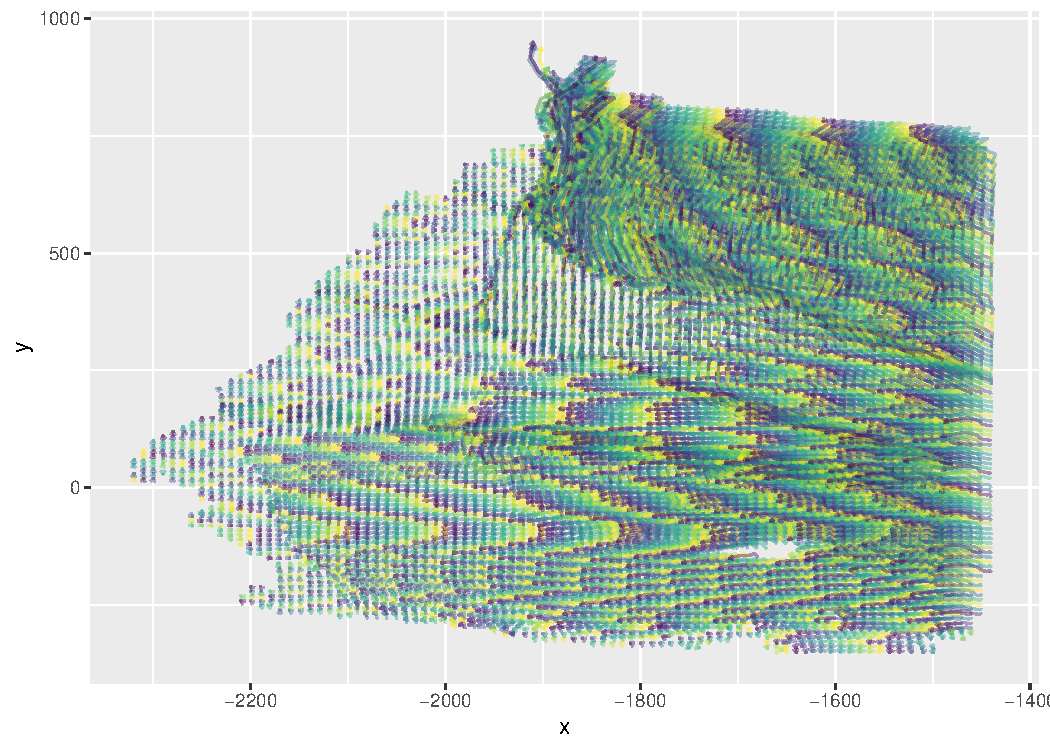
\includegraphics[width=\linewidth,]{spatio-temporal-model-arctic-sea-ice_files/figure-latex/trajectories-1} 

}

\caption{Plot of gpid trajectories over time to show movement and direction of movement of each gpid}\label{fig:trajectories}
\end{figure}

\hypertarget{nonstationary-spatio-temporal-methods}{%
\subsection{Nonstationary Spatio-Temporal
Methods}\label{nonstationary-spatio-temporal-methods}}

\hypertarget{method-motivation}{%
\subsubsection{Method Motivation}\label{method-motivation}}

Since we want to detect cracks only using movement data, it is first
important to visualize the movement. Thus, a plot of the trajectory of
each \(g_j\) is found in \cref{fig:trajectories}. Each line is a
trajectory, \(g_j\), where only its known locations are plotted and
connected. An arrow is also given in order to indicate the direction of
the movement. The coloring of each \(g_j\) does not have a special
meaning, they are just used to distinguish individual trajectories. This
figure shows that groups of trajectories appear to move with similar
patterns. For instance, a the top of \cref{fig:trajectories}, a group of
trajectories are traveling upwards, while in the middle a group is
traveling from right to left. Visualizing the movement led to the idea
of clustering similar trajectories. Each trajectory can be summarized by
a bounding box that represents it's movement over time. This allows for
the creation of features that can be used in a clustering algorithm, and
it circumnavigates the missing data issue. After the bounding box
features are created, the trajectories can be grouped with other that
have similar features. The idea is that ice cracks may form on the
boundary between groups, as these groups are moving differently.

\hypertarget{methods}{%
\section{Methods}\label{methods}}

\hypertarget{spatio-temporal-clustering-bounding-box}{%
\subsection{Spatio-Temporal Clustering: Bounding
Box}\label{spatio-temporal-clustering-bounding-box}}

\hypertarget{bounding-box-features}{%
\subsubsection{Bounding Box Features}\label{bounding-box-features}}

The bounding box that is created around each trajectory is made up of a
number of features that represent it's movement. Features of the
bounding box includes the length traveled between the minimum and
maximum location of a coordinate, representing the total distance
traveled. However, the maximum and minimum locations may not always
correspond to the first and last day of the time frame. Hence, the
difference in each coordinate from the latest observation to the
earliest observation in the time frame was also found. The change from
latest of earliest observation is then used to calculate the angle of
change to find the direction of movement of the trajectory. Further,
since the focus is on the cluster boundaries, we must ensure the
clusters are contiguous, meaning clusters are not co-located across
multiple geographic locations. To ensure some geographic continuity, we
also include the average coordinate values for each trajectory.

A bounding box can be created around a whole trajectory, or for smaller
trajectories. Sub-trajectories may provide more information while
ensuring adequate data is available for the clustering process. A
balance between ensuring data completeness and capturing sufficient
movement is essential. If creating a bounding box for a sub-trajectory,
for instance by week, previous week features may be included as inputs
into the clustering algorithm. This may be done to ensure some
consistency between consecutive time frames, as previous movement may
imapct current movement. After all of the different features are
calculated, the values are then standardized to give each feature
similar weight in the clustering process.

\hypertarget{k-means}{%
\subsubsection{K-Means}\label{k-means}}

To cluster the trajectories we used k-means clustering, which partitions
\(n\) observations into \(k\) clusters, with \(k\) being a pre-specified
number. The goal of this method is to minimize the squared Euclidean
distance between an observation and the centroid vector of a cluster
\citep{steinley_kmeans_2006}. This method requires each observation to
be in a cluster, which is beneficial as we want to know what group each
trajectory is more similar to. However, a drawback of k-means is that
the number of clusters must be known and specified prior to clustering.
We determine the number of clusters using the silhouette statistics,
which compares within cluster distances to between cluster distances
\citep{kodinariya_2013}. Ice movement is a dynamic process, so if
clustering sub-trajectories, like weeks, then we would expect that each
week may have a different number of clusters. Thus, when clustering by
week, the silhouette statistic will be calculated separately for each
week.

\hypertarget{spatio-temporal-interpolation}{%
\subsection{Spatio-Temporal
Interpolation}\label{spatio-temporal-interpolation}}

\hypertarget{finding-spatio-temporal-neighbors}{%
\subsubsection{Finding Spatio-Temporal
Neighbors}\label{finding-spatio-temporal-neighbors}}

\begin{figure}[tbp]

{\centering 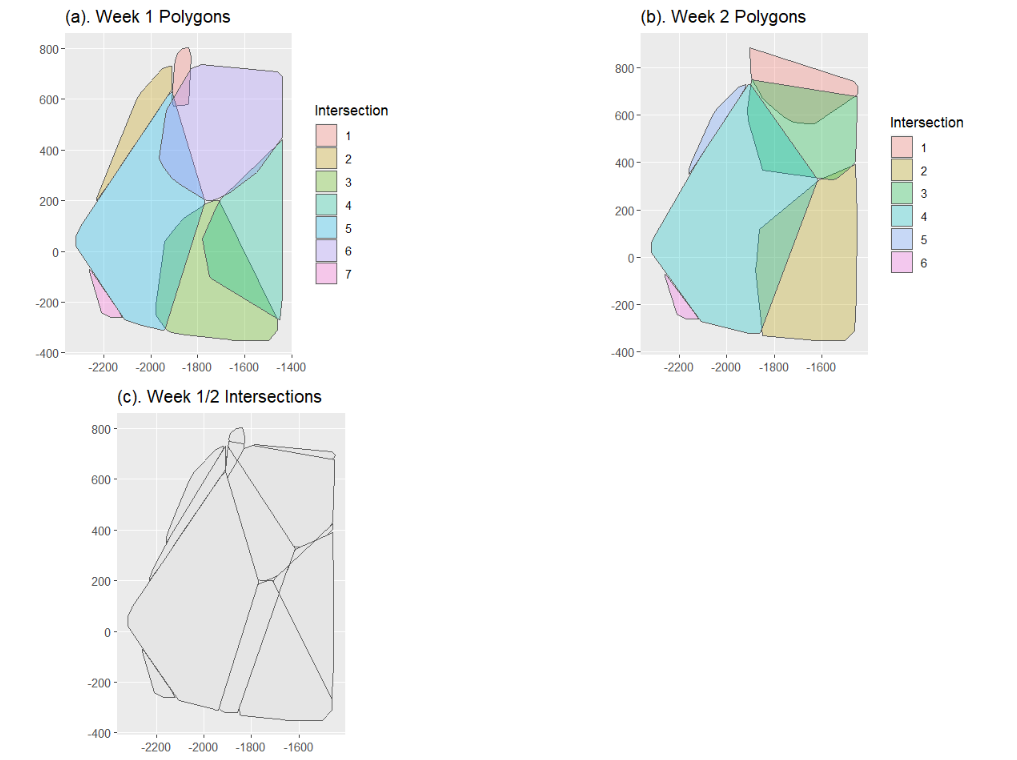
\includegraphics[width=0.8\linewidth,]{images/int-one} 

}

\caption{(a). Polygons of week 1 clusters (b). Polygons of week 2 clusters (c). Intersection polygons of the overlap of week 1 and week 2 polygons}\label{fig:int-plot}
\end{figure}

Due to the data collection method, the data is susceptible to be missing
in chunks due to the path of the satellite. Hence, we want to be able to
interpolate these missing points to have completely gridded data. This
can be challenging due to the lack of close neighbors, as all the data
round a point may also be missing. Additionally, some interpolation
methods are not available due to the non-stationarity of the data, as
the ice is moving in patches.

Our proposed method for interpolation missing locations involves finding
and using spatio-temporal neighbors of the missing identifier. The
clusters determined by the bounding box features can also be used to
identify these spatio-temporal neighbors. Creation of the clusters is
determined by similar movements, so we can use the information given to
us by these clusters to interpolate. Meaning, if we know how points move
in a cluster at a specific time, we can assume a missing identifier in
the same cluster would move similarly. In this method, new clusters are
created for each week. The idea is that the intersection of one week's
clusters with the week before and week after would create groups. Each
member of a group is then a spatio-temporal neighbor of the other
members as they are in a similar geographic location over time.

The first step in finding these intersections is to create polygons for
each cluster. A polygon is created by finding the boundary coordinates
of each of the clusters. In a sequential manner, a polygon is created
around each cluster, generally starting with one on the top edge of the
ice sheet followed by neighboring clusters until there is a polygon for
each cluster. After each polygon is created, then all of the \(g_j\)
located within this polygon are removed from the dataset, even if the
\(g_j\) was assigned to a different cluster. This was done to reduce the
amount of polygon overlapping. Additionally, if a \(g_j\) is classified
to a different cluster than all of it's neighbors, most likely that
\(g_j\) should actually be classified like it's neighbors.

Once we create the polygons for each week, we can find the intersection
of polygons for different weeks to define spatio-temporal neighbors. The
coordinates of the overlapping polygon create an intersection, where the
coordinates also form a polygon. Each \(g_j\) is then assigned to an
intersection based on which intersection coordinates contains its first
observed location of the week. All of the points within that
intersection are considered to be spatio-temporal neighbors since they
are located in a similar geographic region over time. For example, if we
want to interpolate missing data in week 1, would first find its
spatio-temporal neighbors. Since it is the first week, there is no
previous week information, so we can only use week 2 to find neighbors.
Next, we identify the coordinates for the intersecting polygons for
these two weeks. Then, the \(g_j\) located in each intersecting polygon
are spatio-temporal neighbors and will be used to create a model for
interpolation in each of the intersecting polygons. \cref{fig:int-plot}
shows this process with (a) and (b) showing the polygons of the clusters
for week 1 and week 2 respectively, and (c) showing the intersections of
the polygons. Some of the intersection polygons are now shown due to
duplicate intersections (caused by overlapping polygons), but each
\(g_j\) is only assigned to one intersection. If a \(g_j\) is not found
in an intersection, it is then removed from the data during this
process, which is a potential area for improvement. Spatio-temporal
neighbors for week 3 are found using a similar process, with just week
2, as this was the last week in the dataset. Creating the intersecting
polygons for week 2 involved the intersection of it's polygons from both
week 1 and week 3.

To use this interpolation method, a spatial grid encompassing the ice
sheet is created for each day. The grid is used in our model as an
estimation of the initial locations of missing \(g_j\), where the model
will adjust this location using its known neighbors. This size of our
grid cells was chosen for a maximum of four \(g_j\) to be located in a
cell, matching with the initial grid used to track the trajectories. The
centroid of the cell was used to estimate each \(g_j\), so each of the
\(g_j\) located in that cell would have the same initial estimate. We do
not want to use these as the final estimate of our missing locations as
it does not take into account movement.

\hypertarget{univariate-interpolation}{%
\subsubsection{Univariate
Interpolation}\label{univariate-interpolation}}

Once the grid was created for initial location estimates of missing
data, a univariate model was developed for both x and y. These models
were creating using the GpGp package in R, which uses the Vecchia's
Approximation for a Gaussian Process \citep{gpgp_pkg}.
\citet{vecchia1988estimation} developed this approximation for a
Gaussian Process, as generally likelihood methods for the covariance
parameter estimates of the Gaussian Process are computationally
unfeasible. This method approximates the Gaussian Process by writing the
joint density as a product of conditional distributions, where only a
subset of the data is used to create these conditional distributions.
The subset chosen greatly affects the approximation and is formed by
neighbors of the observation. Ordering the the observations by one of
the coordinates determines these neighbors. In
\citet{guinness_permutation_2018}, updates to the ordering process were
developed. A maximum minimum based ordering is used to sort the data
based on sequentially picking the next point that has the maximum
minimum distance to all previously selected points. Then the number of
neighbors used for the subset can be defined and found from this
ordering. Additionally, \citet{guinness_permutation_2018} introduces a
grouping method where groups are determined by partitioning observations
into blocks, and each block's input to the likelihood can be computed at
the same time. These updates were shown to further increase the accuracy
of these models and lower computation time. Further,
\citet{guinness_gaussian_2021}, provides an efficient method for
applying Fisher's scoring to maximize the log-likelihood by developing a
single pass algorithm to compute the Fisher's Information and the
gradient of the Vecchia Approximation. Once again, this was done to help
lower computation time. The updates made in
\citet{guinness_permutation_2018} and \citet{guinness_gaussian_2021} are
implemented in the GpGp package.

In order to fit the model, we need to define:

\begin{itemize}
\tightlist
\item
  Y = x or y. Dimension interested in (univariate response)
\item
  loc = The matrix of x, y, and time (t) of known data. Made of
  locations at the desired time (t), the day before (t-1), and the day
  after (t+1).
\item
  X = Is a matrix of 1's the length of the number of observed data, also
  known as the design matrix.
\item
  m\_seq = A sequence of values for number of neighbors in each subset.
  Our models used a sequence of 10 to min(N-1, 30). Includes N-1 in case
  we have a small number of observations, the model does not try to
  create subset in which it needs more neighbors than there are
  observations.
\end{itemize}

We specified the covariance function as the exponential space-time
covariance function, as defined by the GpGp package documentation
\citep{gpgp_pkg}. It is defined as
\[C(\theta) = \sigma^2e^{-||D^{-1}(x-y)||}. \quad (2)\] where
\[D = \left(\begin{array}{ccccc} 
\phi + c_0 & \\
 & \phi + c_0\\
 &  & \ddots\\
 &  &  & \phi + c_0 \\
 &  &  &  &  \tau+c_0
\end{array}\right). \] The parameters in the covariance function are of
\(\sigma^2\) (variance), \(\phi\) (spatial range), \(\tau\) (temporal
range), and \(c_0\) (nugget). The spatial and temporal ranges are
smoothness parameters that relate to dependence over space and time
respectively. The nugget parameter is the measurement error. The output
is the maximum Vecchia likelihood estimates for the mean and covariance
parameters. The model created by these estimates can be used to predict
the unobserved locations at the time (t). The initial grid estimates of
the x and y values are used as the starting locations in the prediction
function and shifted based on the estimated model parameters.
Predictions for x or y (depending on the Y specified in the fitted
model) are made by finding the conditional expectation of the model
developed.

\hypertarget{simulation}{%
\section{Simulation Study}\label{simulation}}

\hypertarget{data-simulation}{%
\subsection{Data Simulation}\label{data-simulation}}

To test the validity of our methods, we conducted a simulation study.
The data was simulated to mimic the motion of sea ice, where the
movement happens in patches that are driven by external factors.
Separate grids are created to simulate the observed data and the
underlying process that is causing the movement. First, to create the
underlying process, a fine grid is created with each cell vertex
representing a point. This grid is a 30x30 equally spaced grid, which is
a total of 900 points. Next, initial cluster memberships are assigned to
create the patches. For simplicity, the points are assigned into two
clusters, each with an equal number of points. Then, this grid is
shifted seven times, to represent seven days, simulating movement in the
underlying process. The movement at each time step of the grid decreases
over time. This data is then used in the exponential space-time
covariance function (defined in (2)), along with defined parameter
values to simulate a covariance matrix. The covariance function will
have different parameter values for each cluster. Additionally, the
parameter values may also slightly differ for X and Y within a cluster.
The covariance functions and defined mean trend is then used to simulate
a Gaussian Process model of the displacement for each location on the
grid at a time.
Hence,\[ U_{d,c}(s,t) \sim GP(\mu_{d,c}, C_{d,c}(\theta)) \quad (4),\]
where c is the cluster (c=1 or 2), d is the dimension (d=x or y), and
the parameter values for the mean (\(\mu_{d,c}\)) and covariance
function (\(C_{d,c}(\theta)\)) can be found in \cref{tab:parms-table}.
Thus, \(U_{d,c}(s,t)\) gives the displacement, or movement, for each
point on the underlying grid for each day.

After the underlying process is created, a coarse grid representing the
observed data is created in similar fashion to the ice data given by
satellites. This is a smaller grid that is encompassed by the underlying
process. Furthermore, since it is coarser, it is made up of less points.
Each point is represented by \((x_{t,j}, y_{t,j})\), where t is the
time, and j is the identifier used to track the movement (like a gpid).
The initial observed grid values would then be represented as
\((x_{t=0,j}, y_{t=0,j})\). Movement of the observed point is determined
by the value of the nearest point of the underlying process for that
day, determined by Euclidean Distance, to the observed point. Hence,
\[(x_{t,j}, y_{t,j}) = (U^{X}_{t-1,c,g}, U^{Y}_{t-1,c,g}) + (x_{t-1,j}, y_{t-1,j}) \quad (5),\]
where \(U^d_{t,c,g}\) is the underlying process for dimension d (d=X,Y),
cluster c (c=1,2), at time t-1 (t=1,\ldots,7), for grid value \(g\),
which is the closest grid location of the underling process to
\((x_{t-1,j}, y_{t-1,j})\). This process is continued until t=7 in order
to get a final simulated data of a week's worth of data.
\cref{fig:grids-combined} shows the initial grid locations for the
underlying process and observed data together. It also shows the true
cluster membership for each grid location.

In order to evaluate our clustering and interpolation method, three
different data sets were simulated in this manner with slightly
different parameter values, which can be found in
\cref{tab:parms-table}. A plot of the trajectories for each simulation
can be found in \cref{fig:traj-wrap}. In Simulation 1 and Simulation 3,
the trajectories generally start mostly linear, with curvature towards
the end of the week. In Simulation 2, more curvature happens earlier in
the week, with more gradual curves as the week progresses.

\begin{figure}[tbp]

{\centering 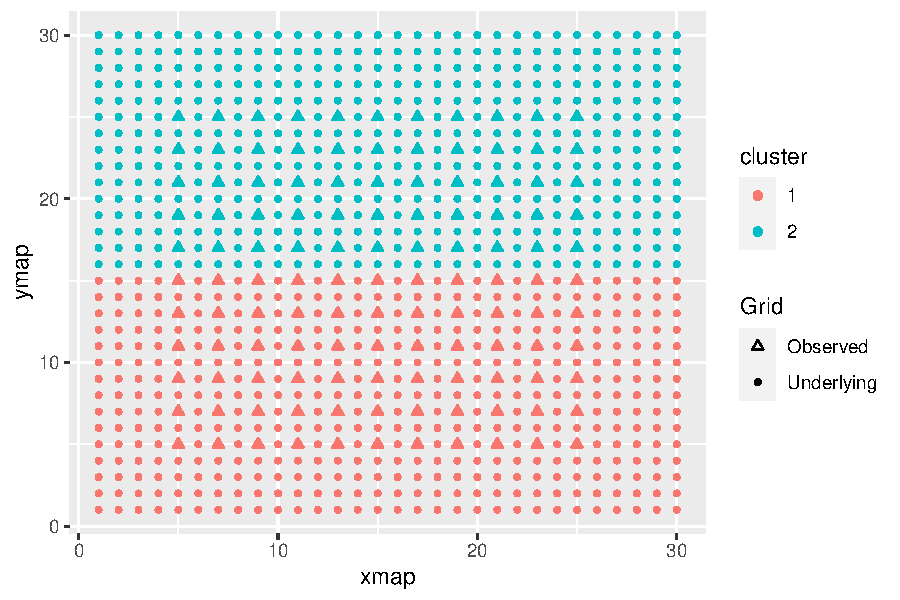
\includegraphics[width=\linewidth,]{spatio-temporal-model-arctic-sea-ice_files/figure-latex/grids-combined-1} 

}

\caption[Simulation Grids]{Underlying Process Grid and Observed Grid together, where the true cluster is also given.}\label{fig:grids-combined}
\end{figure}

\begin{figure}[tbp]

{\centering 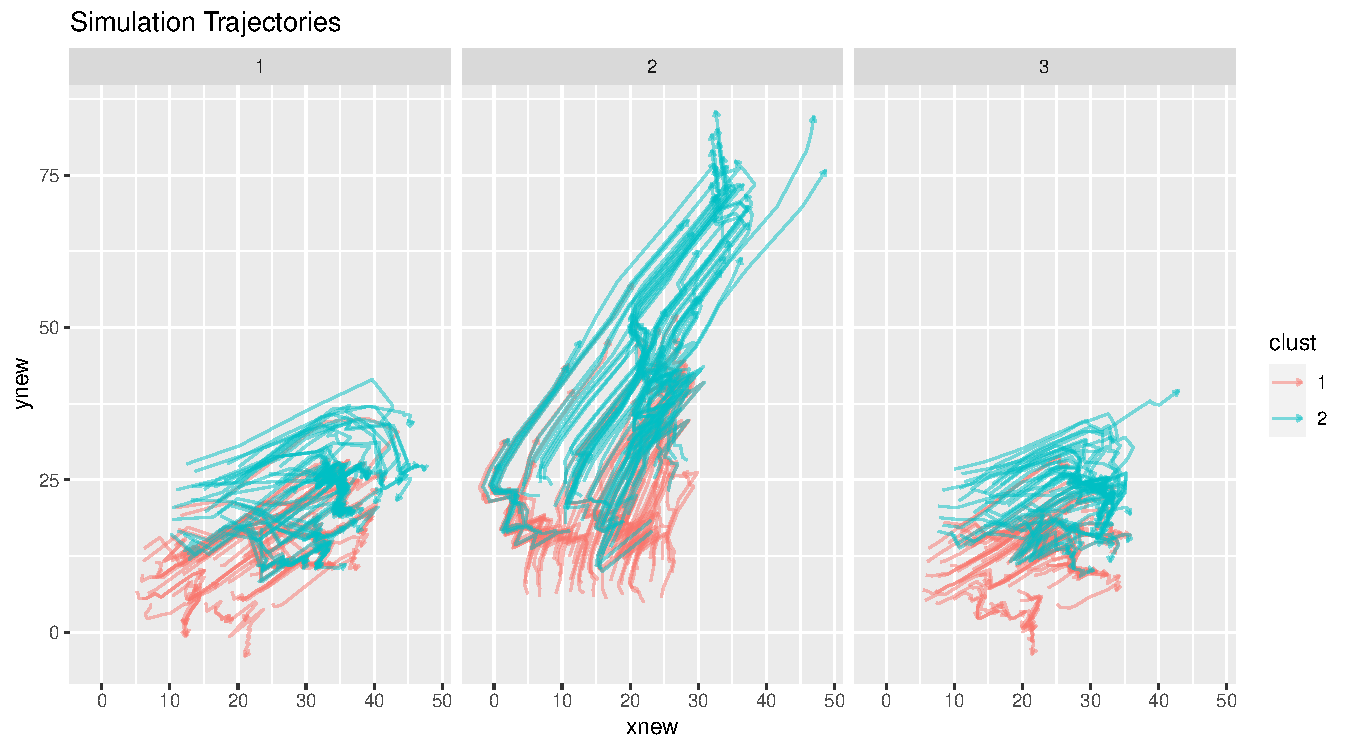
\includegraphics[width=\linewidth,]{spatio-temporal-model-arctic-sea-ice_files/figure-latex/traj-wrap-1} 

}

\caption{Trajectory Plots for each Simulated Data Set }\label{fig:traj-wrap}
\end{figure}

\begin{table}

\caption{\label{tab:parms-table}Parameters Y for Underlying Process for Each Cluster}
\centering
\begin{tabular}[t]{rrrrrrrrrrr}
\toprule
\multicolumn{1}{c}{ } & \multicolumn{5}{c}{X} & \multicolumn{5}{c}{Y} \\
\cmidrule(l{3pt}r{3pt}){2-6} \cmidrule(l{3pt}r{3pt}){7-11}
Cluster & $\sigma^{2}_{x}$ & $\phi_{x,s}$ & $\tau_{x}$ & $Nugget_x$ & $\mu_x$ & $\sigma^{2}_{y}$ & $\phi_{y,s}$ & $\tau_{y}$ & $Nugget_y$ & $\mu_y$\\
\midrule
\addlinespace[0.3em]
\multicolumn{11}{l}{\textbf{Simulation 1}}\\
\hspace{1em}1 & 5 & 5 & 5 & 0 & 2.0 & 5 & 5 & 5 & 0 & 1.5\\
\hspace{1em}2 & 40 & 60 & 10 & 0 & 10.0 & 80 & 50 & 10 & 0 & 6.0\\
\addlinespace[0.3em]
\multicolumn{11}{l}{\textbf{Simulation 2}}\\
\hspace{1em}1 & 1 & 10 & 5 & 0 & 0.5 & 2 & 10 & 7 & 0 & 2.0\\
\hspace{1em}2 & 20 & 20 & 2 & 0 & 2.0 & 25 & 20 & 3 & 0 & 4.0\\
\addlinespace[0.3em]
\multicolumn{11}{l}{\textbf{Simulation 3}}\\
\hspace{1em}1 & 2 & 10 & 5 & 0 & 1.5 & 2 & 10 & 5 & 0 & 1.0\\
\hspace{1em}2 & 20 & 20 & 10 & 0 & 6.0 & 20 & 30 & 10 & 0 & 3.0\\
\bottomrule
\end{tabular}
\end{table}

\hypertarget{clustering-method}{%
\subsection{Clustering Method}\label{clustering-method}}

\begin{figure}[tbp]

{\centering 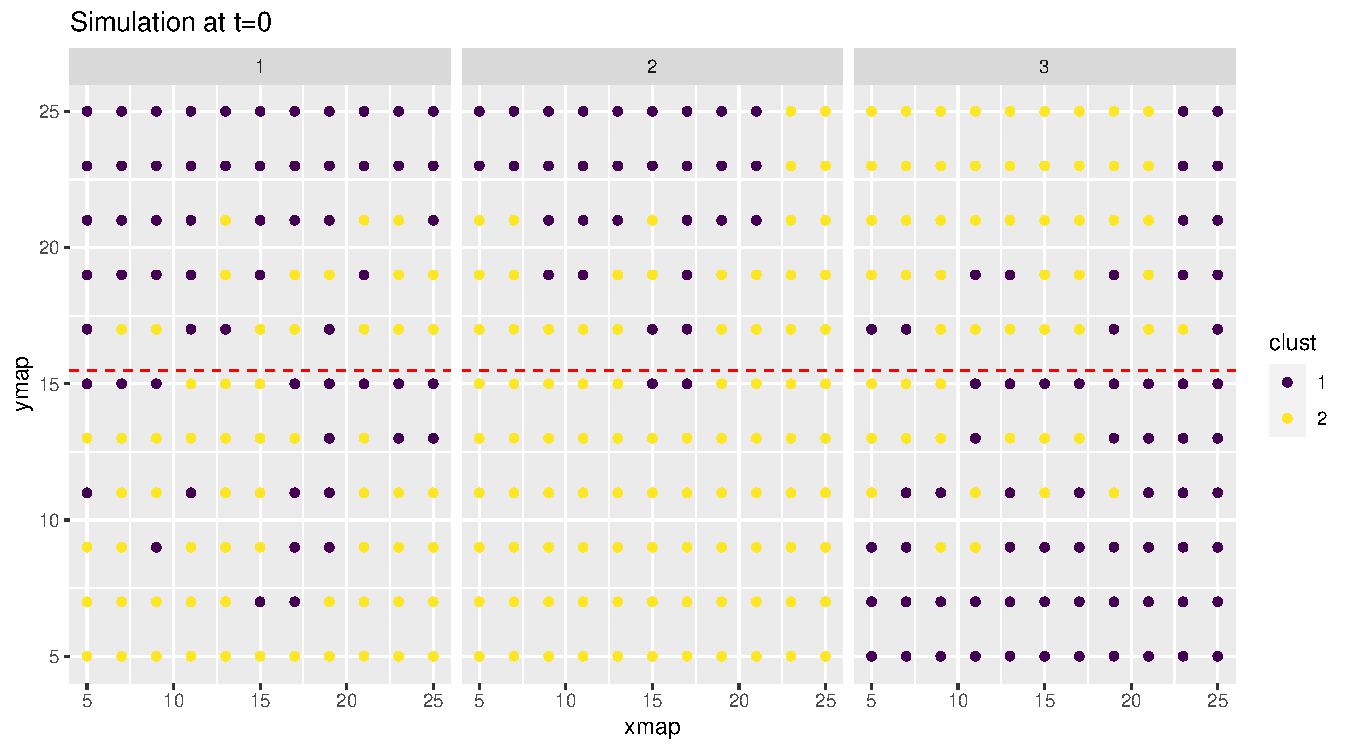
\includegraphics[width=\linewidth,]{spatio-temporal-model-arctic-sea-ice_files/figure-latex/plot-og-clus-1} 

}

\caption{Clusterings of Observed Data on Original Grid}\label{fig:plot-og-clus}
\end{figure}

\begin{figure}[tbp]

{\centering 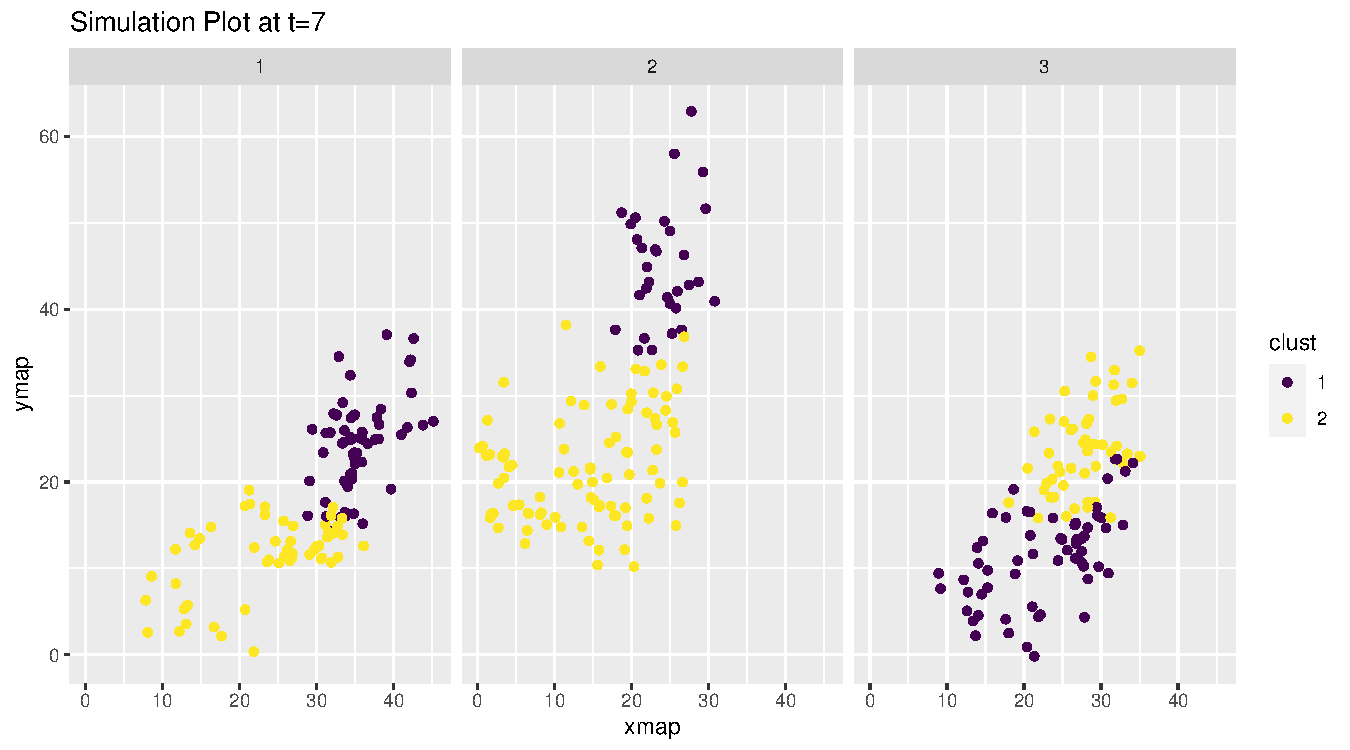
\includegraphics[width=\linewidth,]{spatio-temporal-model-arctic-sea-ice_files/figure-latex/all-clus-1} 

}

\caption{Clusterings of Observed Data on Final Day of Data Set}\label{fig:all-clus}
\end{figure}

Now, our proposed spatio-temporal clustering method, using a bounding
box, is performed on each of the simulated datasets. Since the true
number of clusters is two, two is used as the k input in the k-means
clustering algorithm. The results are shown at two different time
points. First, the k-means determined clusters is visualized on the
initial grid to visualize how well our method performed when can see the
true clusterings (see \cref{fig:plot-og-clus}). The cut-off for the
initial assigned cluster groupings is given by the red-dashed line. In
this figure, a majority of the points seem to be clustered correctly,
however, there are a number of missclassified points in each of the
simulations. In Simulation 1, most of the missclassifications seem to be
along the border, but do seem to increase from left to right. Most of
cluster 2 is clustered correctly in Simulation 2, with the majority of
missclassifications in cluster 1 happening along the edges and boundary.
Similarly, in Simulation 3 most of the missclassifications are near the
border, with a handful along the right edge in cluster 2. If there is a
missclassified point that is surrounded by points correctly classified,
this would be considered a part of the same cluster of its neighbors.
This is due to the desire to have contiguous clusters and we are also
primarily interested in the cluster boundaries. In the future, a
post-processing filter to address these anomalies can be developed.

The second time point where the clusters are visualized is on the last
day of the week in order to see if the clusters determined by the
bounding box can distinguish movement over time. In \cref{fig:all-clus},
there are distinguishable boundaries between clusters for each of the
simulations. Simulation 3 has a little overlap along the boundary, but
can still distinguish between the two clusters. Thus, by clustering
using the movement features of a trajectory, we are able to distinguish
the differences in the movement patterns of the data, where the cluster
boundaries to define the boundaries between the movement patterns. Some
of the missclassifications on the original grid may be due to the fact
that the value for the underlying process that was added to get the new
location was determined by the closest grid cell of the underlying
process by Euclidean distance. If the point eventually becomes closer to
the other cluster, meaning that cluster's underlying process values are
being added to cause the movement, it will eventually start to move like
it. So if it spends more time moving like cluster 1 than cluster 2, as
an example, it will be most likely be classified as cluster 1, even if
that was not what it was initially assigned.

\hypertarget{interpolation-method}{%
\subsection{Interpolation Method}\label{interpolation-method}}

\begin{table}

\caption{\label{tab:results-table}RMSE for Interpolation Methods}
\centering
\begin{tabular}[t]{rrrrrr}
\toprule
\multicolumn{2}{c}{Intersection} & \multicolumn{2}{c}{Linear} & \multicolumn{2}{c}{No Intersection} \\
\cmidrule(l{3pt}r{3pt}){1-2} \cmidrule(l{3pt}r{3pt}){3-4} \cmidrule(l{3pt}r{3pt}){5-6}
$X_{int}$ & $Y_{int}$ & $X_{lin}$ & $Y_{lin}$ & $X_{no int}$ & $Y_{no int}$\\
\midrule
\addlinespace[0.3em]
\multicolumn{6}{l}{\textbf{Simulation 1}}\\
\hspace{1em}1.495585 & 1.516627 & 1.0420551 & 1.2255967 & 1.437696 & 1.294731\\
\addlinespace[0.3em]
\multicolumn{6}{l}{\textbf{Simulation 2}}\\
\hspace{1em}1.628306 & 1.579724 & 1.4546991 & 1.5396450 & 1.473934 & 1.488392\\
\addlinespace[0.3em]
\multicolumn{6}{l}{\textbf{Simulation 3}}\\
\hspace{1em}1.342212 & 1.337799 & 0.9500911 & 0.9206641 & 1.457596 & 1.489168\\
\bottomrule
\end{tabular}
\end{table}

The above simulations are also used to check the performance of our
spatio-temporal interpolation model. For each of the simulations,
another week of data is similarly created and clustered. Polygons for
the two clusters are created. Then, the intersection polygons of the
weeks polygons are found. Once again, an intersections represent the
spatio-temporal neighbors of the data within that intersection polygon.
Next, 10\% of the data for the first week are randomly assigned to be
missing. Then a univariate model for x and y are developed in order to
obtain our estimates of the missing locations. Additionally, in order to
have a baseline to compare our method to, we also ran linear
interpolation on the same data. Linear interpolation estimates an
objects unknown location along a straight-line path between two known
locations. It has been shown to work well for trajectories that follow a
straight-line path and have a lot of sampled points. On the other hand,
it tends to not work as well when a trajectory follows a more curved
path or is not heavily sampled
\citep{wentz_comparison_2003, guo_improved_2021}. A third method was
used for comparison that is similar to our intersection method. Here,
instead of running the model inside an intersection, the intersections
were ignored, and a model was developed using all known points for t-1,
t, and t+1 (this essentially ignores the nonstationarity aspect of our
data). The Root Mean Square Error (RMSE) for each of the simulations and
interpolation methods can be found in \cref{tab:results-table}.

Our interpolation method never seems to outperform linear interpolation.
However, outside of Simulation 3, the results are not very different. In
Simulation 3, running the model for each intersection performs better
than the overall model. Further, since the clusters were created with
different movements, in order to see if there are different areas where
our method may perform better, \cref{tab:results-table-by-clust} breaks
out the RMSE calculations by cluster. In this table, we see similar
results. For Simulation 1, linear interpolation always performs the
best. In Simulation 2, our method outperforms linear interpolation for Y
in cluster 2. However, the model using all the data performs the best
here. Simulation 3 is similar to Simulation 1. Nonetheless, linear
interpolation performing the best may not be surprising, as there are
long periods of linear movement in each of the simulations, so the
results may be dependent on what points where randomly removed.
Additionally, linear interpolation can not estimate the first or last
point of a trajectory, so there are fewer predicted locations used to
calculate the RMSE. Thus, these simulations show that linear
interpolation may generally outperform our method, but our method may
have some promise with curved data that may not be highly sampled. As an
example, in \(Y_{s2,c2}\), the data is more spread out and curved than
the others. The other simulations may have curves, but samples are taken
closer together, or the data may be spread out but mostly is linear. The
results on if creating the intersections is necessary is mixed. However,
these results may be impacted by some of the intersection not containing
much data, which may impact model development. Through the simulations,
we also found that having a fine enough grid for estimates of the
missing data as starting values in the prediction function is key. If
the grid is too coarse, this can impact the accuracy of the estimations.

\begin{table}

\caption{\label{tab:results-table-by-clust}RMSE for Interpolation Methods by cluster}
\centering
\begin{tabular}[t]{rrrrrrr}
\toprule
\multicolumn{1}{c}{ } & \multicolumn{2}{c}{Intersection} & \multicolumn{2}{c}{Linear} & \multicolumn{2}{c}{No Intersection} \\
\cmidrule(l{3pt}r{3pt}){2-3} \cmidrule(l{3pt}r{3pt}){4-5} \cmidrule(l{3pt}r{3pt}){6-7}
Cluster & $X_{int}$ & $Y_{int}$ & $X_{lin}$ & $Y_{lin}$ & $X_{no int}$ & $Y_{no int}$\\
\midrule
\addlinespace[0.3em]
\multicolumn{7}{l}{\textbf{Simulation 1}}\\
\hspace{1em}1 & 1.382578 & 1.555438 & 0.8154561 & 1.1625768 & 1.562165 & 1.290407\\
\hspace{1em}2 & 1.572680 & 1.487765 & 1.1881687 & 1.2722442 & 1.336760 & 1.297965\\
\addlinespace[0.3em]
\multicolumn{7}{l}{\textbf{Simulation 2}}\\
\hspace{1em}1 & 1.699892 & 1.653159 & 1.3158771 & 1.3290263 & 1.657531 & 1.596003\\
\hspace{1em}2 & 1.583802 & 1.533976 & 1.5034563 & 1.6115459 & 1.407423 & 1.450749\\
\addlinespace[0.3em]
\multicolumn{7}{l}{\textbf{Simulation 3}}\\
\hspace{1em}1 & 1.317954 & 1.346376 & 1.1561450 & 1.0959499 & 1.433968 & 1.404708\\
\hspace{1em}2 & 1.353094 & 1.333882 & 0.6469916 & 0.6733144 & 1.484391 & 1.581026\\
\bottomrule
\end{tabular}
\end{table}

\begin{table}

\caption{\label{tab:cp-table-sim}Proportion of Prediction interval containing observed and Average Standard Deviation of Estimates for Simulated Data}
\centering
\begin{tabular}[t]{lrrrr}
\toprule
Simulation & Proportion of X & Avg SD of X & Proportion of Y & Avg SD of Y\\
\midrule
1 & 0.2807018 & 0.3819895 & 0.2982456 & 0.3511526\\
2 & 0.1875000 & 0.4158057 & 0.2500000 & 0.4495713\\
3 & 0.2916667 & 0.3715751 & 0.3750000 & 0.3841953\\
\bottomrule
\end{tabular}
\end{table}

\begin{table}

\caption{\label{tab:cp-sim-table}Proportion of Prediction interval containing observed by Cluster for Simulated Data}
\centering
\begin{tabular}[t]{rrrrrrr}
\toprule
\multicolumn{1}{c}{ } & \multicolumn{2}{c}{Simulation 1} & \multicolumn{2}{c}{Simulation 2} & \multicolumn{2}{c}{Simulation 3} \\
\cmidrule(l{3pt}r{3pt}){2-3} \cmidrule(l{3pt}r{3pt}){4-5} \cmidrule(l{3pt}r{3pt}){6-7}
Cluster & $X_{s1}$ & $Y_{s1}$ & $X_{s2}$ & $Y_{s2}$ & $X_{s3}$ & $Y_{s3}$\\
\midrule
1 & 0.2917 & 0.2083 & 0.3333 & 0.4167 & 0.0667 & 0.2667\\
2 & 0.2727 & 0.3636 & 0.1000 & 0.1500 & 0.3939 & 0.4242\\
\bottomrule
\end{tabular}
\end{table}

A benefit of using a model-based approach to interpolate missing
locations is that we are able to determine the uncertainty of the
estimate. In order to do so, conditional draws of the unobserved values
given the observed values can be used to quantify the uncertainty. This
is accomplished by exploiting an advantage of Vecchia's Approximation
that approximate draws from a Gaussian Process model can be made through
the inverse Cholesky Factor \citep{guinness_permutation_2018}.
Therefore, for each model, 30 simulations of predictions are done and
used to calculate the standard deviation. These can be used to create an
interval of our estimates. The intervals are found by
\(\hat{x} \pm (2*sd_x)\) and \(\hat{y} \pm (2*sd_y)\), where \(\hat{x}\)
and \(\hat{y}\) are the predictions, and \(sd_x\) and \(sd_y\) are the
standard deviations determined by the conditional simulations. Next,
found the proportion of these intervals that contain the true value. For
each simulation, the proportions can be found in
\cref{tab:cp-table-sim}, along with the average standard deviation
values. The proportions in this table are low, mainly in the 20\%-30\%
range. Like the RMSE values, the proportions can be separated by
cluster, which are found in \cref{tab:cp-sim-table}. These values are
also low, with the x values for cluster 1 in Simulation 3 having almost
no intervals that contain the actual value. Finally,
\cref{tab:cp-table-over-under} shows the proportion of intervals that
overestimate or underestimate the actual value. For Simulations 2 and 3,
the x intervals underestimate, whereas the Y intervals are an
overestimate. For Simulation 1, the proportion of overestimates is
slightly higher than the underestimates for Y-values, but almost
identical for x.

\hypertarget{results}{%
\section{Results}\label{results}}

\begin{figure}[tbp]

{\centering 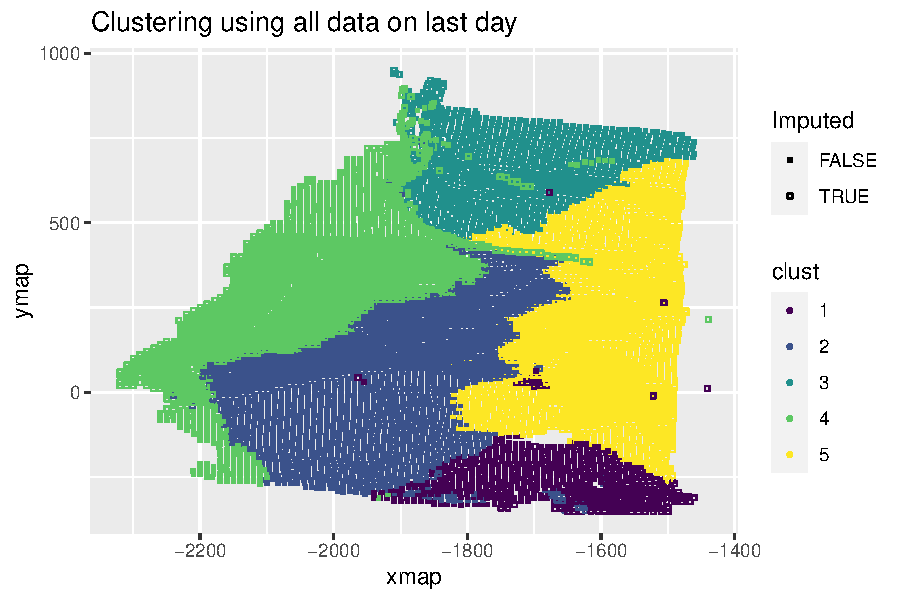
\includegraphics[width=\linewidth,]{spatio-temporal-model-arctic-sea-ice_files/figure-latex/ex-result-1} 

}

\caption{Results of Clustering using Bounding Box Method for all the Data}\label{fig:ex-result}
\end{figure}

\begin{figure}[tbp]

{\centering 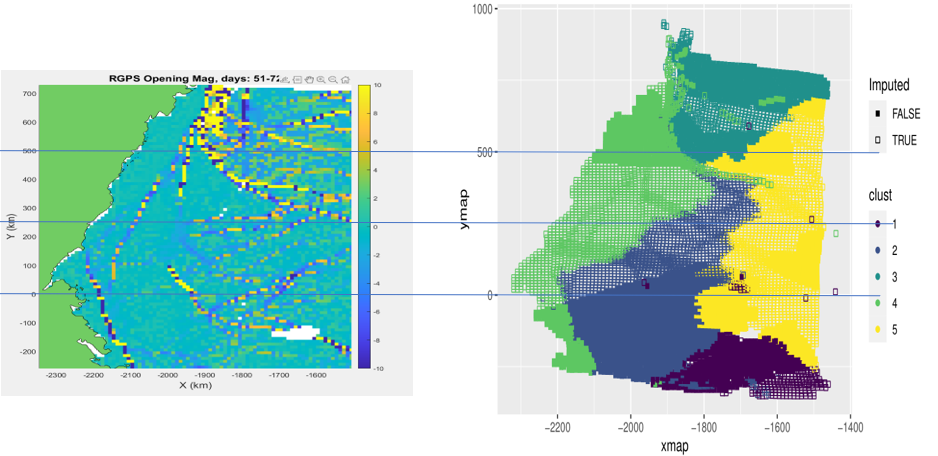
\includegraphics[width=1\linewidth,]{images/all_weeks_comp_correct} 

}

\caption{Comparison of our method to results of a previous method, which find cracks using a kinematic algorithm}\label{fig:all-week-comp}
\end{figure}

The simulation results showed some promise for our methods, so next the
methods are applied on the ice motion dataset.

\hypertarget{clustering-using-all-data}{%
\subsection{Clustering Using All Data}\label{clustering-using-all-data}}

First we used our spatio-temporal clustering method by creating bounding
boxes around the full trajectory of each gpid. Once the bounding box
features are created and standardized, the number of clusters were
determined using the silhouette statistic. This silhouette statistic for
the full trajectory data suggested five clusters to be appropriate. The
results from the clustering algorithm are shown in \cref{fig:ex-result}.
In \cref{fig:ex-result}, each of the colors represent one cluster; each
of the squares represent a gpid. The locations of the gpids on this map
are determined by its last observed location in the data set. We
hypothesize that cracks in the sea ice will be found along the
boundaries of the clusters as those gpids have different movements. In
the middle of some of the clusters, there are some singular gpids whose
cluster membership does not match its neighbors. These gpids in
practicality will belong to the same clusters as its neighbors and a
crack is not considered to have formed here.

To see how well our method is performing, we can compare it to other sea
ice crack detection algorithms. One such method is by plotting the
deformation data using a kinematic crack algorithm calculated using the
RGPS data \citep{peterson_evaluating_2011}. \cref{fig:all-week-comp}
gives a comparison of our bounding box clustering method and the
kinematic crack algorithm using side-by-side graphs. It is important to
note that this image does not represent the true ice cracks, just the
cracks determined by this method. The larger cracks, which are
represented by the yellow and dark blue lines are more certain. The
graphs are aligned so that their axes match up for easier comparison.
The lines given in the left figure are derived from the opening
magnitude of the ice sheet. Most of the figure has a color around zero,
denoting no opening, whereas potential large cracks are found with the
dark blue or yellow. Many of our cluster boundaries match up with the
cracks identified by the kinematic crack algorithm, though we are
limited due to the number of clusters. For example, on the bottom left
side of both plots, we see a line that goes down and to the right. At
the bottom right of both plots, we see a line moving through the hole in
the gpids. Additionally, towards the top of both figures, we see a
curved boundary that starts at the top of the ice sheet and moves to the
bottom left in a curved manner.

\hypertarget{clusterings-by-weeks}{%
\subsection{Clusterings By Weeks}\label{clusterings-by-weeks}}

Since trajectories can be long, it may also be useful to look at
sub-trajectories, as we may lose information by clustering the whole
trajectory, which may impact results. We split the data into three
separate weeks. Through some testing of our methods, we found that by
week was the smallest time period we could successfully cluster, as
anything smaller led to large changes in the clusterings between each
weeks (unstable). We would expect the weeks to have different
clusterings, but would also expect there to be some continuity between
them. The clusters by week can be found in
\cref{fig:by-week-cluster-plot}, where can see some similarities in
clusters over time.

With these weekly clusters we can also compare them similarly to
\cref{fig:all-week-comp}, instead manipulating the days used to create
the magnitudes by the proper weeks time frame. Additionally, we had a
picture from Day 66 of our data set, which gives an image of recurring
leads based on visible and infrared Advanced Very High Resolution
Radiometer (AVHRR) data \citep{lead_pic_2009}. \cref{fig:week-comp},
includes grid lines to aid in comparison of the pictures, due to the
aspect ratios not aligning perfectly. One major cracks stands out in
both images. Our boundary between cluster 1 and 3 aligns until about
(-1880,400), at this point our boundary curves in more steeply.
Eventually, the upper section of the cluster boundary between clusters 5
and 6 continue the crack. Additionally, we can see some of the lighter
cracks in our graph. For example, we can also see another curved
boundary above the one just discussed, and can see one on the bottom
left, similar to what was seen in \cref{fig:all-week-comp}.

\begin{figure}[tbp]

{\centering \includegraphics[width=\linewidth,]{spatio-temporal-model-arctic-sea-ice_files/figure-latex/by-week-cluster-plot-1} 

}

\caption{Results of Clustering using Bounding Box Method by Week}\label{fig:by-week-cluster-plot}
\end{figure}

\begin{figure}[tbp]

{\centering 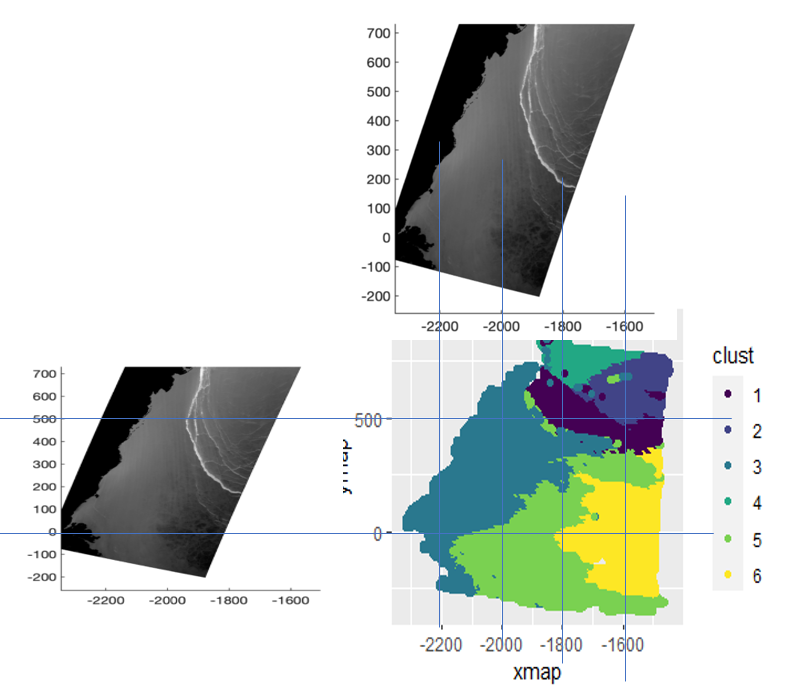
\includegraphics[width=1\linewidth,]{images/week-comp} 

}

\caption{Comparison of our method to results of a previous method for Week 3}\label{fig:week-comp}
\end{figure}

\hypertarget{univariate-interpolation-1}{%
\subsection{Univariate Interpolation}\label{univariate-interpolation-1}}

\begin{figure}[tbp]

{\centering 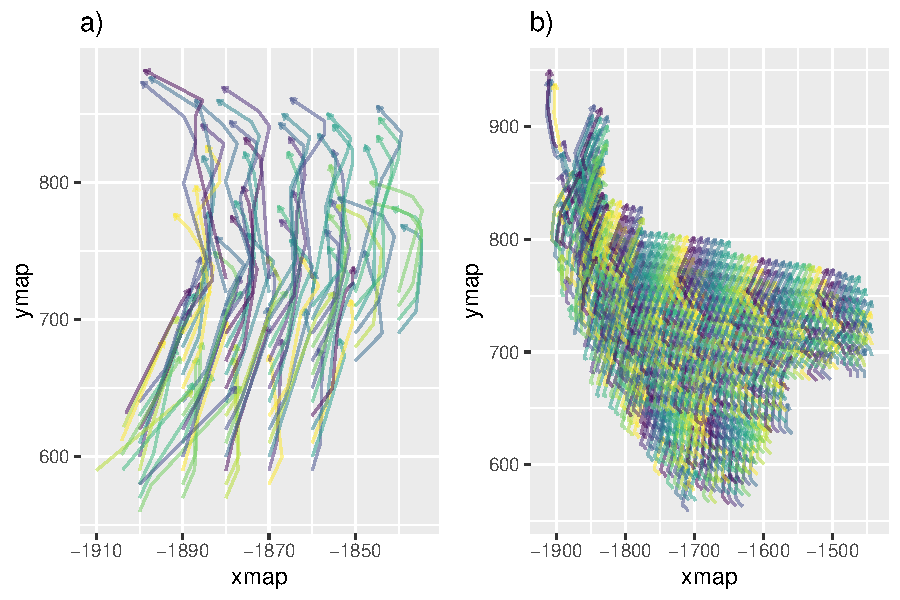
\includegraphics[width=\linewidth,]{spatio-temporal-model-arctic-sea-ice_files/figure-latex/int-best-plots-1} 

}

\caption{Trajectories for a) Week 2 Cluster 1, where our method peforms best and b) Week 2 Cluster 5, where linear interpolation performs best. These are instances where our method outperforms linear interpolation}\label{fig:int-best-plots}
\end{figure}

\begin{table}

\caption{\label{tab:results-table2}RMSE for Interpolation Methods}
\centering
\begin{tabular}[t]{rrrrrr}
\toprule
\multicolumn{2}{c}{Intersection} & \multicolumn{2}{c}{Linear} & \multicolumn{2}{c}{No Intersection} \\
\cmidrule(l{3pt}r{3pt}){1-2} \cmidrule(l{3pt}r{3pt}){3-4} \cmidrule(l{3pt}r{3pt}){5-6}
$X_{int}$ & $Y_{int}$ & $X_{lin}$ & $Y_{lin}$ & $X_{noint}$ & $Y_{noint}$\\
\midrule
\addlinespace[0.3em]
\multicolumn{6}{l}{\textbf{Week 1}}\\
\hspace{1em}3.156499 & 3.239215 & 1.526844 & 4.179299 & 3.092995 & 3.067393\\
\addlinespace[0.3em]
\multicolumn{6}{l}{\textbf{Week 2}}\\
\hspace{1em}3.142291 & 3.061897 & 2.000556 & 1.398822 & 3.197890 & 3.150918\\
\addlinespace[0.3em]
\multicolumn{6}{l}{\textbf{Week 3}}\\
\hspace{1em}3.178118 & 3.093726 & 1.026822 & 1.214958 & 3.190372 & 3.150259\\
\bottomrule
\end{tabular}
\end{table}

Next, we tested our spatio-temporal interpolation method on the ice
movement dataset in order to see how it performs on real data. We did
not predict on the already missing data in the dataset for validation
purposes. For cross validation, we can create a model for an
intersection and time. In a the intersection and time combination, 10\%
of the known data were removed from the dataset. Next, we found all of
the observed data in that intersection for t-1, t, and t+1 in order to
obtain the spatio-temporal neighbors. Then, using the observed data, the
model was fit and used to estimate the missing data points. This was
then done for all intersection and time combinations for the three
weeks. The total RMSE for each week can be found in
\cref{tab:results-table2}. Additionally, linear interpolation and the
model with no intersection was performed on the same missing data for
comparison, like what was done for the simulated data. However, since
linear interpolation is unable to estimate data without a point before
or after (essentially the beginning or end of the week), it is not
exactly a one-to-one comparison. Also, for the no intersection model,
models were able to be created for each day for Week 2 and Week 3, but
were only able to create a model for one day in Week 1 due to the
log-likelihood failing to converge. So, the Week 1 RMSE value for this
week is not useful for comparison. In \cref{tab:results-table2}, for the
most part, linear interpolation looks to outperform the other methods,
except for Y-values in Week 1.

However, when looking at the trajectory plot in \cref{fig:trajectories},
can see that some of the trajectories in the plot are more linear than
others (ie. have different movements defined by the clusters). Based on
our simulation study, our method may have some improvement over linear
interpolation on curved data and less-sampled trajectories. Thus, the
RMSE values are additionally broken out by cluster, as these are the
groups of movement patterns in the data. These values can be found for
each week in \cref{tab:results-clust1-actual},
\cref{tab:results-clust2-actual}, and \cref{tab:results-clust3-actual}.
Once again, linear interpolation generally outperforms our method, but
there are two exceptions. For Week 1 and Week 2, linear interpolation
performed the worst of the other two methods for Cluster 1. In
\cref{fig:by-week-cluster-plot}, Cluster 1 for both of these weeks is at
the top of the plot. When comparing this cluster location to the
trajectory plot in \cref{fig:trajectories}, the top of the figure looks
to be where the most curved movement happens with longer distance
traveled over time. So linear interpolation may not work as well here.
Further, \cref{fig:int-best-plots} and \cref{fig:lin-best-plots}, zoom
in on examples where our intersection model method performs best and
linear interpolation performs the best respectively. When comparing both
figures, our method seems to perform better on longer trajectories, as
observed points are more spread out along the trajectory.

As previously stated, though the RMSE for the non-intersection model was
lower than the intersection model in week 1, this number is only
representing one day's worth of data. So for Cluster 1 in week 1, our
proposed method seems to be performing the best. For week 2 cluster 1,
there mixed results between the two model methods, as one performs
better for x and the other for y. When comparing the two model-based
approaches, find mixed results when compare their performance, but the
intersection model performs better more often. These results, once
again, shows that our method has some promise with non-linear and
less-sampled data.

\begin{table}

\caption{\label{tab:results-clust1-actual}RMSE by Cluster for Week 1 for Interpolation Methods}
\centering
\begin{tabular}[t]{rrrrrrr}
\toprule
\multicolumn{1}{c}{ } & \multicolumn{2}{c}{Intersection} & \multicolumn{2}{c}{Linear} & \multicolumn{2}{c}{No Intersection} \\
\cmidrule(l{3pt}r{3pt}){2-3} \cmidrule(l{3pt}r{3pt}){4-5} \cmidrule(l{3pt}r{3pt}){6-7}
Cluster & $X_{int}$ & $Y_{int}$ & $X_{lin}$ & $Y_{lin}$ & $X_{noint}$ & $Y_{noint}$\\
\midrule
1 & 0.6279070 & 0.4651163 & 3.198509 & 13.0416159 & 2.515490 & 3.410473\\
2 & 0.1711712 & 0.1909091 & 0.186626 & 0.3586513 & 4.257679 & 4.105569\\
3 & 0.3716012 & 0.3154574 & 1.314808 & 3.0661913 & 2.162818 & 2.883046\\
4 & 0.3116090 & 0.3299389 & 1.396271 & 2.4424844 & 2.459404 & 2.777074\\
5 & 0.0634328 & 0.2603774 & 0.770609 & 3.1659150 & 3.895142 & 3.241075\\
\addlinespace
6 & 0.2432046 & 0.3261803 & 1.888726 & 5.6371115 & 2.597491 & 3.098273\\
\bottomrule
\end{tabular}
\end{table}

\begin{table}

\caption{\label{tab:results-clust2-actual}RMSE by Cluster for Week 2 for Interpolation Methods}
\centering
\begin{tabular}[t]{rrrrrrr}
\toprule
\multicolumn{1}{c}{ } & \multicolumn{2}{c}{Intersection} & \multicolumn{2}{c}{Linear} & \multicolumn{2}{c}{No Intersection} \\
\cmidrule(l{3pt}r{3pt}){2-3} \cmidrule(l{3pt}r{3pt}){4-5} \cmidrule(l{3pt}r{3pt}){6-7}
Cluster & $X_{int}$ & $Y_{int}$ & $X_{lin}$ & $Y_{lin}$ & $X_{noint}$ & $Y_{noint}$\\
\midrule
1 & 3.003332 & 2.934830 & 3.2398842 & 3.3166785 & 2.625197 & 3.043491\\
2 & 2.943829 & 2.889240 & 2.5484750 & 1.0259089 & 2.889908 & 2.939434\\
3 & 2.937204 & 2.901313 & 1.5772293 & 1.9941807 & 2.946309 & 3.030898\\
4 & 3.255739 & 3.127827 & 1.4045887 & 0.5231723 & 3.452124 & 3.190633\\
5 & 4.205982 & 4.159416 & 0.3144192 & 0.3723263 & 4.413450 & 4.202641\\
\bottomrule
\end{tabular}
\end{table}

\begin{table}

\caption{\label{tab:results-clust3-actual}RMSE by Cluster for Week 3 for Interpolation Methods}
\centering
\begin{tabular}[t]{rrrrrrr}
\toprule
\multicolumn{1}{c}{ } & \multicolumn{2}{c}{Intersection} & \multicolumn{2}{c}{Linear} & \multicolumn{2}{c}{No Intersection} \\
\cmidrule(l{3pt}r{3pt}){2-3} \cmidrule(l{3pt}r{3pt}){4-5} \cmidrule(l{3pt}r{3pt}){6-7}
Cluster & $X_{int}$ & $Y_{int}$ & $X_{lin}$ & $Y_{lin}$ & $X_{noint}$ & $Y_{noint}$\\
\midrule
1 & 2.848267 & 2.852569 & 2.0407810 & 2.6713539 & 2.700013 & 3.049005\\
2 & 2.806052 & 2.951553 & 2.1528308 & 2.0588226 & 2.649236 & 2.852982\\
3 & 3.657974 & 3.593269 & 0.1858682 & 0.4401472 & 3.759902 & 3.594164\\
4 & 2.675125 & 2.777055 & 1.5252900 & 0.7179780 & 2.871803 & 2.919869\\
5 & 3.162914 & 3.037071 & 0.2051635 & 0.4789511 & 3.079266 & 3.095375\\
\addlinespace
6 & 3.209643 & 3.010415 & 0.2811618 & 0.5534701 & 3.227123 & 3.005055\\
\bottomrule
\end{tabular}
\end{table}

The proportion of the prediction intervals containing the observed data,
along with the average standard deviations are given for the ice data in
\cref{tab:cp-table}. These values were found in the same way as the
simulated data. The standard deviations are higher than what was seen
with the simulated data, but the proportions are similar (ranging from
25\%-31\%). Once again, this can be broken down by cluster in
\cref{tab:cp-clust-actual}. However, none of the large proportions are
as large as would b desired, but in cluster 1, week 1 the proportion for
X is above 50\%, with the proportion for Y close to 50\%.

\begin{table}

\caption{\label{tab:cp-table}Proportion of Prediction interval containing observed and Average Standard Deviation for Ice Data}
\centering
\begin{tabular}[t]{lrrrr}
\toprule
Week & Proportion of X & Avg SD of X & Proportion of Y & Avg SD of Y\\
\midrule
1 & 0.2779244 & 0.8341885 & 0.3122212 & 0.9207825\\
2 & 0.2631451 & 0.7538514 & 0.3041575 & 0.8136070\\
3 & 0.2466216 & 0.7597185 & 0.2640766 & 0.7950100\\
\bottomrule
\end{tabular}
\end{table}

\begin{table}

\caption{\label{tab:cp-clust-actual}Proportion of Prediction interval containing observed by Cluster for Ice Data}
\centering
\begin{tabular}[t]{rrlrrrr}
\toprule
Cluster & $W1_{x}$ & $W2_{x}$ & $W3_{x}$ & $W1_{y}$ & $W2_{y}$ & $W3_{y}$\\
\midrule
1 & 0.6279 & 0.3873 & 0.3843 & 0.4651 & 0.3757 & 0.3983\\
2 & 0.1712 & 0.2973 & 0.4367 & 0.1909 & 0.3456 & 0.3376\\
3 & 0.3716 & 0.3022 & 0.1679 & 0.3155 & 0.3373 & 0.2039\\
4 & 0.3116 & 0.2184 & 0.4327 & 0.3299 & 0.2674 & 0.3365\\
5 & 0.0634 & 0.1268 & 0.2207 & 0.2604 & 0.1185 & 0.2409\\
\addlinespace
6 & 0.2432 & NA & 0.1587 & 0.3262 & NA & 0.2243\\
\bottomrule
\end{tabular}
\end{table}

Next, instead of a random hold-out of all of the data, we took a random
hold-out of points along cluster borders. We are interested in points
along the cluster border as those might be locations of irregular
movement. Boundaries are defined in the code as points where some of its
neighbors are from a different cluster. Otherwise the process remains
the same as before. \cref{tab:border-cv-rmse} contains the RMSE values
for our method and linear interpolation. The model with all the data (no
intersection) is not used for comparison here as these models produced
an error with issues in convergence of the log-likelihood. When just
look at the weeks overall, our model only outperforms linear
interpolation in Week 1 for y-values. Furthermore, this was broken out
by cluster in \cref{tab:border-clust}. This shows similar results as the
random hold-out, with our method outperforming linear interpolation in
cluster 1 for Week 1 and 2. Additionally, in Week 1, our method performs
best for y-values for all clusters expect for cluster 2. Once again, it
should be noted that linear interpolation cannot estimate points if
nothing before or after it, so we are working with less data in the RMSE
calculation.

As in prior sections, 30 conditional simulations were performed in order
to calculate the uncertainty. Using the standard deviation found from
these simulations we calculated an interval. Then the proportion of
intervals that contain the true value are calculated
(\cref{tab:cp-table-border}). The average standard deviation values are
also given to give an idea of typical interval width. Once again, as in
\cref{tab:cp-table}, these values are low, with most intervals not
containing the true value. In \cref{tab:cp-table-border-clust}, these
values are broken out by cluster. The values do seem slightly higher in
the instances where our method performs best, but still low. Finally, in
\cref{tab:cp-table-border-ou}, found if the true values tend to be over
or under the interval. Our interval is an underestimate of the true
values, but still a high percentage of our interval is still an
overestimate.

\begin{table}

\caption{\label{tab:border-cv-rmse}RMSE for Interpolation Methods on Cluster Border Points}
\centering
\begin{tabular}[t]{rrrr}
\toprule
\multicolumn{2}{c}{Intersection} & \multicolumn{2}{c}{Linear} \\
\cmidrule(l{3pt}r{3pt}){1-2} \cmidrule(l{3pt}r{3pt}){3-4}
$X_{int}$ & $Y_{int}$ & $X_{lin}$ & $Y_{lin}$\\
\midrule
\addlinespace[0.3em]
\multicolumn{4}{l}{\textbf{Week 1}}\\
\hspace{1em}3.215281 & 3.407760 & 1.6062169 & 4.494381\\
\addlinespace[0.3em]
\multicolumn{4}{l}{\textbf{Week 2}}\\
\hspace{1em}3.296520 & 3.255547 & 2.0389810 & 1.832126\\
\addlinespace[0.3em]
\multicolumn{4}{l}{\textbf{Week 3}}\\
\hspace{1em}3.031460 & 2.957910 & 0.9913019 & 1.240117\\
\bottomrule
\end{tabular}
\end{table}

\begin{table}

\caption{\label{tab:border-clust-tab}RMSE by Cluster for Cross Validation Along Cluster Borders}
\centering
\begin{tabular}[t]{rrrrrrrrrrrrr}
\toprule
\multicolumn{1}{c}{ } & \multicolumn{4}{c}{Week 1} & \multicolumn{4}{c}{Week 2} & \multicolumn{4}{c}{Week 3} \\
\cmidrule(l{3pt}r{3pt}){2-5} \cmidrule(l{3pt}r{3pt}){6-9} \cmidrule(l{3pt}r{3pt}){10-13}
Cluster & $X_{int}$ & $Y_{int}$ & $X_{lin}$ & $Y_{lin}$ & $X_{int}$ & $Y_{int}$ & $X_{lin}$ & $Y_{lin}$ & $X_{int}$ & $Y_{int}$ & $X_{lin}$ & $Y_{lin}$\\
\midrule
1 & 2.380 & 3.903 & 2.351 & 8.327 & 2.808 & 3.044 & 3.819 & 5.192 & 2.687 & 2.863 & 1.883 & 2.618\\
2 & 4.010 & 4.344 & 0.191 & 0.251 & 2.940 & 2.962 & 2.388 & 0.989 & 2.738 & 2.848 & 1.879 & 1.916\\
3 & 2.794 & 3.135 & 1.140 & 3.882 & 2.936 & 3.067 & 1.456 & 1.972 & 3.490 & 3.308 & 0.218 & 0.434\\
4 & 2.488 & 3.005 & 1.236 & 4.317 & 3.258 & 3.202 & 1.318 & 0.537 & 2.843 & 3.223 & 2.255 & 1.458\\
5 & 4.161 & 3.865 & 0.623 & 4.546 & 4.138 & 3.878 & 0.431 & 0.336 & 2.838 & 2.832 & 0.216 & 0.490\\
\addlinespace
6 & 3.194 & 3.299 & 2.214 & 4.848 & NA & NA & NA & NA & 3.205 & 2.921 & 0.303 & 0.561\\
\bottomrule
\end{tabular}
\end{table}

\begin{table}

\caption{\label{tab:cp-table-border}Proportion of Prediction interval containing observed and Average Standard Deviation for Ice Data}
\centering
\begin{tabular}[t]{lrrrr}
\toprule
Week & Proportion of X & Avg SD of X & Proportion of Y & Avg SD of Y\\
\midrule
1 & 0.320 & 0.942 & 0.344 & 1.069\\
2 & 0.267 & 0.808 & 0.267 & 0.871\\
3 & 0.277 & 0.775 & 0.283 & 0.785\\
\bottomrule
\end{tabular}
\end{table}

\begin{table}

\caption{\label{tab:cp-table-border-clust}Proportion of Prediction interval containing observed by Cluster for Cluster Border}
\centering
\begin{tabular}[t]{rrrllrr}
\toprule
\multicolumn{1}{c}{ } & \multicolumn{2}{c}{Week 1} & \multicolumn{2}{c}{Week 2} & \multicolumn{2}{c}{Week 3} \\
\cmidrule(l{3pt}r{3pt}){2-3} \cmidrule(l{3pt}r{3pt}){4-5} \cmidrule(l{3pt}r{3pt}){6-7}
Cluster & $X_{s1}$ & $Y_{s1}$ & $X_{s2}$ & $Y_{s2}$ & $X_{s3}$ & $Y_{s3}$\\
\midrule
1 & 0.592 & 0.592 & 0.467 & 0.413 & 0.422 & 0.357\\
2 & 0.270 & 0.288 & 0.28 & 0.278 & 0.471 & 0.418\\
3 & 0.347 & 0.312 & 0.337 & 0.351 & 0.184 & 0.245\\
4 & 0.482 & 0.301 & 0.26 & 0.251 & 0.491 & 0.309\\
5 & 0.157 & 0.300 & 0.149 & 0.163 & 0.283 & 0.264\\
\addlinespace
6 & 0.273 & 0.396 &  &  & 0.177 & 0.254\\
\bottomrule
\end{tabular}
\end{table}

\hypertarget{discussion}{%
\section{Discussion}\label{discussion}}

Our Bounding Box clustering method was developed to group trajectories
by their movement, and to compensate for missing data. This method was
shown through simulations and actual data that the boundaries of the
clusters determined by the trajectory movements provide a reasonable
estimation of the location of cracks. However, a major drawback of this
method is that since the k-means clustering approach is used, our method
relies on a pre-defined number of clusters, which is typically unknown.
Furthermore, with having a set number of clusters, there is a limit on
how many cluster boundaries representing cracks that can be identified.
Thus, not all possible leads will be identified. Our method seems
suggest that other approaches to clustering may be useful to extend this
method in order to identify higher resolution cracks. Also, our method
provides information about how the ice sheet is moving, which may also
be important when developing climate models.

Through our simulations and the use of the ice movement data, we have
demonstrated some situations where our interpolation method may be
beneficial. First, it takes into account the nonstationarity of the
data, which generally shows slight improvement over using all the data
to develop the model. Instances where the intersection model under
performs the other model may be due to lack of data to develop a better
model at that intersection. Secondly, it showed improvements, in terms
of RMSE, over linear interpolation for curved and not highly sampled
data with the ice data. Additionally, our method is able to estimate
missing locations on the first and last day of a dataset when linear
interpolation is not able to. Another benefit of our method is that
since a model is created, we are able to get an uncertainty measure with
the predictions. Our method should eventually be tested against curved
methods, like cubic splines, to see if it will outperform simpler,
curved-based methods. Despite the benefits our method, linear
interpolation outperformed our proposed method in most cases. So using
the additional information about the movement does not provide any
benefit if the trajectories follow a linear pattern and only interested
in location estimation.

An issue with our interpolation approach is that when creating the
intersections, if an object is not located within a spatial-temporal
intersection, it is removed from the data used to develop the models, as
only developing models within intersections. Thus, we could be losing
valuable information to obtain the estimates. Typically this only
happens to gpids on the edges of the ice pack.

When it comes to developing the models with the Vecchia Approximation,
some other issues arise. The first is that when the temporal range is
large, especially in comparison with the spatial range, the model is not
able to be developed as the log-likelihood does not converge. Generally
when this happens the last Fisher Scoring iteration before the error has
an exceptionally large temporal range value. Additionally, the
covariance parameters estimated by the model do not seem to make sense
practically even when the model can be successfully fit because all the
parameter values outside of the nugget are large, even though the
variance and spatial range values are sometimes more reasonable for the
simulated data. For example, the large temporal range means that the
data is not changing over time, and that there is a strong dependence
over multiple lifetime's worth of data, which is probably not realistic.
Using the simulated data as an example, in Simulation 1 the Y values for
cluster two were generated with \(\sigma^2\) = 80, \(\phi\) = 50,
\(\tau\) = 10, \(c_0\)= 0. The values estimated for the model in
intersection 3, time 3 were \(\sigma^2\) = 77.91, \(\phi\) = 458,
\(\tau\) = 686,239.164, \(c_0\) = 0. In this scenario, the model is
overestimating the spatial and temporal range parameters, with the
temporal range being a much larger overestimate. This may be due to only
working with a small amount of data that is not moving much over time.
This is especially true when looking at the ice sheet data. With the
simulated data, as more days were added to the datasets used to create
the clusters and defines the intersections, the temporal range does
slowly decrease. Also, \citet{guinness_gaussian_2021} points out that
when the range parameter estimates are much larger than the maximum
distance between points, which we see with our data, the likelihood
function has a hard time jointly identifying the range parameters and
variance, causing issues in the calculation of our model. With the
simulation data, we tried setting a value for the covariance parameters
and found that if set \(\phi\), then \(\tau\) is still large. On the
other hand, if set \(\tau\), then \(\phi\) is closer to the true value.
Showing that the temporal dependence is posing an issue, which may be
due to lack of days and lack of movement over the days.

Another potential source for error when using a space-time covariance
function is that variation in time is needed. Otherwise, if we only have
observed data for one day of the three days used to create the models,
the model is unable to be developed. Another issue, that was mainly seen
in the models without the intersection in Week 1, the location columns
were sometimes considered too linearly dependent to form a model.
Generally, taking a random subset of the data allowed a model to
converge. Finally, sometimes the estimated model can be developed, but
an error occurs in the prediction. This occurs when we only have one
location to estimate, as the nearest neighbor approach is used when
computing the conditional estimates of the prediction. Thus, we need at
least two missing points to create an estimate.

\hypertarget{conclusion}{%
\section{Conclusion}\label{conclusion}}

Sea ice plays a vital role in the Earth's energy balance, as when cracks
form in the ice, warm air from the ocean is released into the
atmosphere. In order to determine where these cracks may form using only
the movement of the ice sheet, a bounding box is created around each
tracked trajectory and the features of the bounding box are used as
input into k-means. Once each gpid is assigned a cluster, a plot of the
results is created where the cluster boundaries would be the location
where ice cracks may form. This method seemed to identify similar cracks
as other ice crack detection methods. Next, using the information from
the clusters, created a model for interpolation from spatio-temporal
neighbors of the missing points. While linear interpolation typically
outperforms our method, we showed some benefit with nonlinear and not
highly sampled data.

In the future, we want to determine the number of clusters through
something other than the silhouette statistic. For example,
\citet{ossama_extended_2011} has a process for determining the number of
unique directions, which may be a better estimate of k. Secondly, more
work needs to be done in the univariate model development for the
interpolation to facilitate convergence in a wider range of situations.
Next, we would like to further investigate a bivariate interpolation
model to estimate both x and y at the same time. Finally, at the moment
our method is a two step process: find clusters and create model in each
cluster. Eventually, we would like to turn this into a one step process,
potentially using voronoi tessellations and a piecewise Gaussian
Process.

\bibliographystyle{agsm}
\bibliography{bibliography.bib}


\end{document}
